\documentclass[11pt]{article}

% \usepackage[sort]{natbib}
\usepackage[style=verbose]{biblatex}
\usepackage{fancyhdr}
\usepackage{graphicx,caption,subcaption,color,float} %Graphics stuff
\usepackage{hyperref,amssymb,amsmath, amsfonts, amsthm, enumerate, bm}
\usepackage{placeins, cancel, wrapfig, xcolor, array, multirow, booktabs, algorithm, algpseudocode} 
\usepackage[margin=0.9in]{geometry}
\usepackage{ulem}
\graphicspath{ {figs/} }
\bibliography{references}

% you may include other packages here (next line)
\usepackage{enumitem}
\usepackage{dirtytalk}

\usepackage{pythonhighlight}

%----- you must not change this -----------------
\topmargin -1.0cm
\textheight 23.0cm
\parindent=0pt
\parskip 1ex
\renewcommand{\baselinestretch}{1.1}
\pagestyle{fancy}
\renewcommand{\theenumi}{\Alph{enumi}}
\makeatletter
\newcommand{\distas}[1]{\mathbin{\overset{#1}{\kern\z@\sim}}}%
\newsavebox{\mybox}\newsavebox{\mysim}
\newcommand{\distras}[1]{%
  \savebox{\mybox}{\hbox{\kern3pt$\scriptstyle#1$\kern3pt}}%
  \savebox{\mysim}{\hbox{$\sim$}}%
  \mathbin{\overset{#1}{\kern\z@\resizebox{\wd\mybox}{\ht\mysim}{$\sim$}}}%
}
\makeatother
%----------------------------------------------------

% enter your details here----------------------------------
\lhead{}
\chead{}
\rhead{}
\lfoot{}
\cfoot{}
\rfoot{}
\setlength{\fboxrule}{4pt}\setlength{\fboxsep}{2ex}
\renewcommand{\headrulewidth}{0.4pt}
\renewcommand{\footrulewidth}{0.4pt}


\title{Homework 1}
\author{Deepak Akhare}

\begin{document}

\maketitle

\textbf{Problem 1:}
Katz centrality

\begin{equation}
    c_{Katz} = \beta (\textbf{I} - \alpha \textbf{A})^{-1} \Vec{1}
\end{equation}

By definition: $\alpha > 0$

For the convergence of Katz centrality, we need to seek for $\alpha$ such that $(I - \alpha \textbf{A})^{-1}$ does not diverge, i.e., the inverse of $(I - \alpha \textbf{A})$ should exist, which requires

\[ det(\textbf{A}-\alpha^{-1}\textbf{I}) \neq 0 \]

However for Eigen-value matrix $\Lambda$

\[ det(\textbf{A}-\Lambda\textbf{I}) = 0 \]

The first value of $\alpha$ that makes this determinant 0 is
\[ \alpha = \frac{1}{\lambda_{max}} \]

Therefore, 
\begin{equation}
     0 < \alpha < \frac{1}{\lambda_{max}}
\end{equation}

will be a sufficient condition for the convergence of Katz centrality

\clearpage


\textbf{Problem 2:}

Number of walk of size 2 from $v_i$ to $v_j$ that go through $v_k\in V$ is

\begin{equation}
    N^{(2)}_{ij} = \sum_{k=1}^n A_{ik}A_{kj} = [A^2]_{ij}
\end{equation}

A walk of size 2 from $v_i$ to $v_j$ that go through $v_k\in V$ clearly means that $v_k$ is the neighbor of both $v_i$ and $v_j$. Therefore the total number of common neighbors $|N(v_i) \cap N(v_j)|$ between nodes $v_i$ and $v_j$ is 

\begin{equation}
    |N(v_i) \cap N(v_j)| = N^{(2)}_{ij} = \sum_{k=1}^n A_{ik}A_{kj} = [A^2]_{ij}
\end{equation}


% \begin{equation}
%     |N(v_i) \cap N(v_j)| = \{v_k | A_{ki}*A_{kj} \neq 0, v_k\in V\}
% \end{equation}

\clearpage

\textbf{Problem 3A:}

program to compute Jaccard’s similarity matrix S

\begin{python}
A = nx.adjacency_matrix(G)
S = np.zeros_like(A.todense(), dtype=float)
for i in range(A.shape[0]):
    for j in range(A.shape[0]):
        S[i,j] = np.array((sum(A[:,i].multiply(A[:,j])) /
        len((A[:,i]+A[:,j]).nonzero()[0])).todense())[0][0]
\end{python}

program to calculate edge between ”Ginori” family and other families in the Florentine Families graph

\begin{python}

new_edges, metric = [], []
for v in Ginori_dict:
    u = 'Ginori'
    p = Ginori_dict[v]
    G.add_edge(u, v)
    print(f"({u}, {v}) -> {p:.8f}")
    new_edges.append((u, v))
    metric.append(p)

\end{python}

Updated program for plotting

\begin{python}

# -- plot Florentine Families graph
nx.draw_networkx_nodes(G, nodelist=nodes, label=nodes, pos=layout, node_size=600)
nx.draw_networkx_edges(G, edgelist=new_edges, pos=layout, edge_color='gray', width=4)

ne = nx.draw_networkx_edges(G, edgelist=new_edges, pos=layout, edge_color=np.asarray(metric), width=4, alpha=0.7)
plt.colorbar(ne)
plt.axis('off')
plt.savefig('similarity.png')

\end{python}


\clearpage

\textbf{Problem 3B:}

\begin{figure}[!h]
    \centering
    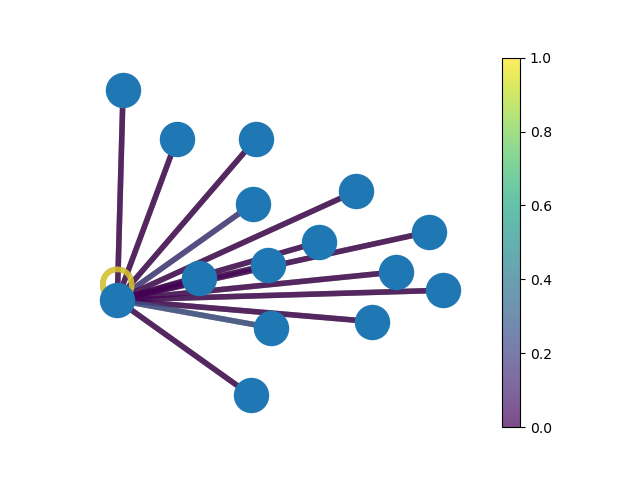
\includegraphics[width = 0.8\textwidth]{similarity.png}
    \caption{Similarity between ”Ginori” family and other families in the Florentine Families graph}
    \label{fig:my_label}
\end{figure}

\clearpage



\end{document}